Pathfinding systems which operate on regular grids are commonly found in modern video games.
Some recent examples include \emph{Company of Heroes} (Relic Entertainment, 2006), \emph{Dawn of War II} (Relic
Entertainment, 2009) and \emph{Dragon Age: Origins} (BioWare, 2010).
Additionally, regular grids often appear in academic literature; for example in areas such as robotics \cite{choset05} and
single-agent pathfinding \cite{yap02,botea04,sturtevant07,harabor08}.
\par
In the context of single-agent pathfinding, and real-time video games in particular, it is often the case that queries sent to
the pathfinding system  need to be solved as quickly as possible.
Traditionally, this requirement is met in one of two ways: (i) by reducing the size of the search space through hierarchical 
decomposition or (ii) through the development of improved heuristics to guide search.
In the case of hierarchical decomposition, techniques such as
HPA*~\cite{botea04} and PRA*~\cite{sturtevant05} seek to construct and explore
a much reduced approximate state space.
These methods are fast and require no significant extra-memory when compared to the classical
A* algorithm \cite{hart68}.
However, they have the disadvantage that solutions are not guaranteed to be optimal.
Meanwhile, in case of the improved heuristics, it has been frequently shown
that obtaining better informed results than than the popular
Manhattan heuristic usually incurs significant memory overhead 
\cite{sturtevant09,goldberg05,Cazenave:06,bjornsson06}.
Furthermore it is well known that even heuristics which differ from perfect information 
by at most a (small) additive constant, can still exhibit poor performance on a range of 
problems such as AI planning and graph search \cite{helmert08,pohl77}.
\par
Very recently a third method for speeding up search has emerged: symmetry breaking \cite{pochter10,harabor10}.
This approach recognises that there are often many paths of identical length between arbitrary pairs of tiles on a map.
The main idea then is to decompose the search space in such a way that, given a particular pathfinding problem, it is possible to
discard from consideration tiles which are on a path of identical length to the one ultimately returned as the solution\footnote{
As we will see, this process also has the added advantage of discarding tiles 
that cannot appear on any optimal path.}.
Algorithms of this type have been  shown to produce results that are not only optimal but also memory efficient, 
particularly when compared with memory-based heuristics.
Additionally, they can significantly improve the search-time performance of the classical A* algorithm; making it competitive,
on certain types of maps, with suboptimal methods such as HPA* and PRA*.
\par
In this work we present Perimeter Search; a new symmetry breaking search algorithm which generalises the method described in \cite{harabor10}.
That work uses an Empty Rooms decomposition (see Figure \ref{fig-overview}) to convert an arbitrary grid map into an
equivalent grid map where only tiles on the perimeter of each empty room, and never the interior, need to be explored during search. 
Though effective, the method is limited to 4-connected grid maps where only straight moves, and not diagonal, are
allowed.
We extend their approach to 8-connected grid maps, which are much more common, and show how the higher branching factor associated 
with this domain makes effective symmetry elimination more challenging.
In the process we develop two novel methods for reducing the branching factor during search.
The first is an offline pruning technique that minimises the size of the perimeter associated with an empty room.
The second is an online optimisation which speeds up node expansion by selectively evaluating either all neighbours
associated with a particular tile or only a subset.
We show that in each case both optimality and completeness are preserved.
We then evaluate our technique experimentally on a number of synthetic and realistic benchmarks, including one well known set 
from the popular roleplaying game \emph{Baldur's Gate II}.
On our test data the average performance of A* is increased by up to 9 times on 8-connected grid maps and up to
18 times on 4-connected grid maps, depending on the topography of the map being used.

\begin{figure}[tb]
       \begin{center}
                       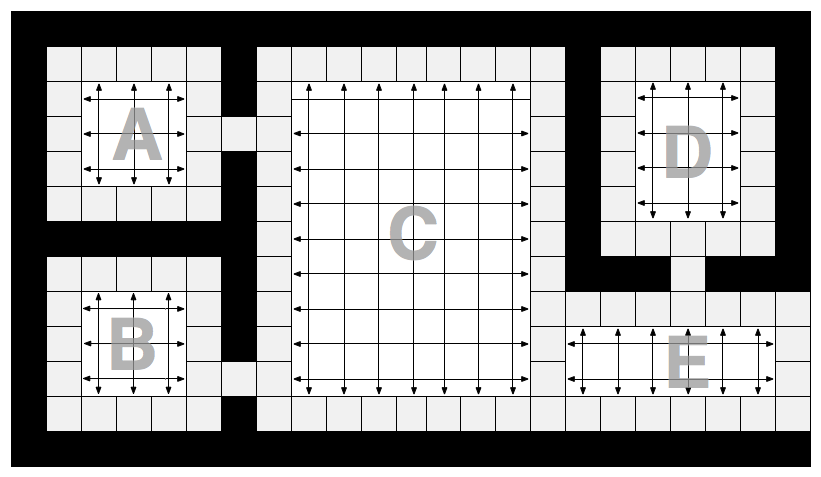
\includegraphics[scale=0.30, trim = 10mm 10mm 10mm 0mm]{diagrams/overview.png}
       \end{center}
	\vspace{-3pt}
       \caption{(Top) A highly symmetric pathfinding instance. Many solutions exist; we highlight three. 
				(Bottom) The same map with the Empty Rooms symmetry elimination method applied. 
				The map is decomposed into a set of obstacle-free rooms from which are pruned all nodes except those on the perimeter.
				They are replaced with a small set of macro edges that connect the perimeter nodes directly.}
       \label{fig-overview}
\end{figure}
